\chapter{Structural predictors of species survival in complex ecological communities} \label{chp:2}
We have commented that explaining the emergence of biodiversity in ecological communities has been a long-standing challenge. In Chapter~\ref{chp:1}  we tackled this issue by introducing a model of intransitive competition, which highlighted how local spatial interactions can lead to stable coexistence. However, despite that  coexistence has been long sought after in ecological systems, environmental perturbations and temporal changes can cause species to go extinct. Observations about the drivers behind species' extinction have significant consequences for biodiversity dynamics and conservation issues. With this in mind, our focus in this Chapter will be on identifying what structural factors better explain extinctions. To do so, we increase our scale of description and model communities at the level of species, which is the unit in which we assess biodiversity.\\

 Over the years, the structure of the network of species interactions has proven to play a crucial role in the stability and resilience of ecosystems, so it is a natural place to look for a priority list of which species to protect \cite{Holme2021NetworksConsequences}. Since the structure arises from the position of the species in the interaction network, a recurrent approach is to rank the species according to some topological measure \cite{McDonald-Madden2016UsingEcosystems,Keyes2021AnLosses}. Some works investigate also other characteristics besides topological features, such as ecological functions \cite{Jordan2008IdentifyingNetworks} or connectance after deletion \cite{Torres-Alruiz2013AIndexes}. A follow-up approach has been to combine these indices \cite{ Gouveia2021,Estrada2007CharacterizationSpecies} and estimate their relative importance, measuring correlations or using machine learning \cite{Gouveia2021}.\\

However, in these topological approaches, two important aspects intrinsic to ecosystems are often neglected. First, the dynamics that are embedded in the network of interactions. Species abundances naturally fluctuate through time, especially if exogenous events like perturbations or species removal occur. The above research usually studies the bare network structure, removing species and their links at discrete time steps, without taking abundance evolution into account. Secondly, there is a bias towards focusing mainly  on trophic interactions \cite{Allesina2009GooglingCoextinctions,Estrada2007CharacterizationSpecies,Keyes2021AnLosses,Torres-Alruiz2013AIndexes,Jordan2008IdentifyingNetworks,Gouveia2021} or ``extended'' food webs, which include resources \cite{Bellingeri2013RobustnessResources} or ecosystem services \cite{McDonald-Madden2016UsingEcosystems} --benefits that humans derive from nature such as food.\\

One explanation for these tendencies may be the fact that studying the relationship between the structure and dynamics of networks, on one side, and more types of interactions, on the other, complicate both the empirical and theoretical analysis. Nevertheless, including other kinds of interactions (such as non-trophic ones) has proven to radically change our understanding  of ecosystems \cite{pocock2012robustness, Fontaine2011TheNetworks, Kefi2015NetworkShores, Garcia-Callejas2018ThePersistence,kefi2012more,bartomeus2021experimental}. Furthermore, in the stage of uncertainty that we are entering with climate change, it is more important than ever to understand how to maintain biodiversity. While predictions of the effects of climate change on species typically focus on its direct impact on individual species, the influence of species interactions should not be overlooked. Species interactions can significantly affect the propagation of this impact to other organisms at all levels by altering community structure and dynamics \cite{gilman2010framework}. \\

In this Chapter, we take a step in the direction of integrating these missing ingredients in the context of environmental change. We aim to discover what are the structural properties that have the species that survive in a community with several types of interactions simultaneously. More specifically, we study what are the structural characteristics that better predict the fate of species whose abundances are evolving in a community where both competition and mutualism are present and that have suffered a perturbation. These non-trophic interactions are thought to play a crucial role in biodiversity and shape the interaction network's architecture \cite{Wang2021InterspecificNetworks,Gracia-Lazaro2018TheEcosystems,bastolla2009mutualism,pocock2012robustness}. We not only include several types of interactions, but also a population dynamics over several underlying network structure. Our analysis encompasses  diverse structures, from  random models to empirical networks, and different interaction intensities to simulate changes in the environment. Moreover, the importance of these structural characteristics, which we define as ``structural predictors'' in the sequel, is ultimately quantified by a decision tree, a type of machine learning algorithm. \\

We find that when only one type of interaction is considered, a single predictor can predict species survival. 
%We find that traditional communities with only one kind of interaction, i.e. only mutualism or only competition, have a single predictor. 
This predictor is different for each type of interaction but it is preserved through the studied network topologies. However, there is no universal predictor when multiple types of interactions are present within the same network. In that sense, each community is unique and has a particular set of node characteristics to assess their species' vulnerability. The set is usually composed of measures that combine network structure with the strength and sign of the interactions. This contrast of results emphasizes how crucial it is to consider the various types of interaction and their strength to advance our understanding of ecological communities.


\begin{comment}
NB: We are studying communities, not ecosystems. \\
papers mainly from: https://docs.google.com/spreadsheets/d/1bq7Vr6msYC6TfhEUPycKtHFvbeKh-8Kq1DP-7Io-qZA/edit?usp=sharing

\textbf{AIM:}
We aim to discover what are the structural characteristics that have the species that survive after an environmental change.

\textbf{IMPORTANCE:} 
- for ecosystems' management: ''these would then be a priority list of what nodes to protect '' from \cite{Holme2021NetworksConsequences}

\textbf{NOVELTY}: key \textbf{differences} with our approach:
0) Usually, do not take dynamics into account, only structure.
1)  when there is dynamics, they run the dynamics until it has stabilized and them, perturb the system. our approach is radically different, as we do not care on the previous equilibrium (does it even exist). We start our simulations right after the perturbation.
2)  Moreover, this perturbation is  usually targeted, ie ''let's remove one random species'' or ''from high to low degree'' or ''one by one''... We let the dynamical system to extinct species.
3) we study several interactions ''at the same time'': mutualism and competition, no food webs!

\textbf{definitions to explain}=
	- persistence
    - make clear what we mean by structure (sometimes called topology) ''positional properties of its species''

\textbf{previous works:}
Lots of works only focus on \textbf{structure without dynamics}, also known as topological approach:
	- they study vulnerability to extinction cascades: \cite{Allesina2009GooglingCoextinctions,Sole2001,Keyes2021AnLosses,Bellingeri2013RobustnessResources,Donohue2017LossCascades}). 
	- and species/ecosystem service/management  action  ranking according to some measure: \cite{Estrada2007CharacterizationSpecies,McDonald-Madden2016UsingEcosystems,Jordan2008IdentifyingNetworks,Keyes2021AnLosses}

Some other papers \textbf{combine structural indices} \cite{ Gouveia2021,Estrada2007CharacterizationSpecies} but in order to estimate the importance, they just correlate (except \cite{Gouveia2021} that uses ML but only with structural measures), we a DT, finer.
- some papers look also at other characteristics of the species besides simple topological features:
		- \textbf{function}\cite{Jordan2008IdentifyingNetworks}
        - \textbf{connectance} after deletion \cite{Torres-Alruiz2013AIndexes} (they call them ''dynamics'')

Focus mainly on 
- \textbf{foodwebs} \cite{Allesina2009GooglingCoextinctions,Estrada2007CharacterizationSpecies,Keyes2021AnLosses,Torres-Alruiz2013AIndexes,Jordan2008IdentifyingNetworks,Gouveia2021} 
- and ''extended food webs''(FW+servises \cite{McDonald-Madden2016UsingEcosystems}, FW+resources \cite{Bellingeri2013RobustnessResources}).	

but... Studying  \textbf{several types of interaction}s (in a community) makes more difficult to find universal structural predictors of survival after an environmental change. necessity and dangers of studying multiple interactions at a time!
	- kefi \cite{Kefi2015NetworkShores}
    -callejas 2018 \cite{Garcia-Callejas2018ThePersistence}
    - from hugo: In ecology, however, there have been
few empirical examples that have considered multiple types
of interactions within the same network, probably because
of the high logistic effort involved in documenting all the
potential interactions present within a community (Melián
et al. 2009, Pocock et al. 2012). Furthermore, the analysis
of these networks presents some difficulties over the analysis
(like the use of multilayer networks, Mucha et al. 2010,
Boccaletti et al. 2014, Kivelä et al. 2014).

\textbf{Concepts that are related}: cascades of extinctions, robustness, perturbations, fragility, vulnerability to species losses, keystone species.
\end{comment}


\section{Ecological communities model}

%We study the impact of the structural properties of a species on its survival in a community that  includes several interaction types simultaneously.  
Our communities consist of $n$ species that can interact mutualistically as well as competitively. Not every species interacts with each other, but the interactions create a complex network (described in Section~\ref{chp2:2.1}). Every species is characterized by its frequency $x_i$, which is influenced by its mutualistic and competitive interactions following a replicator dynamics (Section~\ref{chp2:2.2}). The structural properties that will be tested as possible predictors of survival are defined in Section~\ref{chp2:2.3}, and the algorithm to test their predictive importance is presented in Section~\ref{chp2:2.4}.

\subsection{Structure: Artificial and Empirical Ecological Networks  } \label{chp2:2.1}

We use networks to describe the structure of the interactions in ecological communities. Each node represents a species, and links document the presence of an interaction. The links can be positive (mutualistic) or negative (competitive) since our subjects of study are communities governed by non-trophic interactions. The nature of the interactions also makes it appropriate to set undirected links, contrary to trophic networks.\\

 Being our main objective to study real communities, we beguin with the construction of simple artificial networks and then build up adding realism till studying, in the end, empirical networks. The parameters of the network models have been set to match those of the empirical counterparts, and to be large enough to provide enough statistics. 

\subsubsection{Random networks}
We have chosen three random models to mimic different connection patterns. Their topologies represent particular properties of how species can interact. As outlined in Section~\ref{chp:methods:networks} of our methods, we will employ the following network models: Erdös-Rènyi model, which serves as null model of ecological networks; the Barabasi-Albert model, which has a scale-free degree distribution; and the Holme-Kim model, which is more realism because presents clustering among species. While the Barabasi-Albert model creates tree-like structures that may not capture the common motifs in nature,  clustering is especially relevant for competitive communities with intransitive or diffuse competition  \cite{godoy2017intransitivity,losapio2019perspectives}, and networks that integrate different interaction types \cite{kefi2016structured} like plant spatial association networks \cite{Saiz2017EvidenceNetworks}.

%\paragraph{1) Erdös-Rènyi model:}  The first studied network structure is the Erdös-Rènyi graph \cite{erdos1959random}, where nodes are connected at random according to a linkage probability $p$. It is typically used  as a null model because the properties of its nodes behave nicely around well-defined average values.
%\paragraph{2) Barabasi-Albert model:} The second step in complexity is to simulate scale-free networks. The underlying motivation is the fact that the presence of generalists and specialists tend to create heavy-tail degree distributions. In particular, we have implemented the preferential attachment model of Barabasi-Albert \cite{Albert2002StatisticalNetworks}. 
%\paragraph{b) Holme-Kim model:} To add up more realism, we use the Holme-Kim model \cite{Holme2002GrowingClustering} because it grants clustering among the species. The previous scale-free model creates tree-like structures that may not represent the common motifs usually present in nature. Especially, competitive communities with intransitive or diffuse competition  \cite{godoy2017intransitivity,losapio2019perspectives}, and networks that integrate different interaction types \cite{kefi2016structured} like plant spatial association networks \cite{Saiz2017EvidenceNetworks}.
 
\subsubsection{Empirical networks}
Along with the artificial networks, we also test our results against different empirical networks representing competitive and mutualistic assemblages. Specifically, we use two different datasets, each one applying a different technique to build the interaction networks. By doing so,  we prevent our results from being biased towards a particular method for inferring interactions. The criteria for choosing these networks have been that they should be connected and have a large number of species, as both conditions ensure well-defined node properties. A complete list of the networks can be found in  Table \ref{tab:empnetworks}. 

\paragraph{(A) Pollination and seed-dispersal networks:} We have chosen networks based on interaction frequencies from the open database of ``Web of Life'' \cite{weboflife}. 
%The networks have only two types (guilds) of nodes (e.g. plants and pollinators, or plants and seed-dispersers), and mutualistic links are only set between nodes of different guilds. 

The networks consist of two types of nodes, $A$ and $B$, that  interact positively with one another. If $N_A$ and $N_B$ denote the number of species in each set, then $n = N_A + N_B$ is the total number of species. These sets represent guilds, for example, plants and pollinators, or plants and seed-dispersers. Mutualistic interactions are only present between nodes of different guilds, and therefore they are fully encoded in a bipartite matrix. 

To infer competition among species that use a common resource, we have supposed (following the logic of the works  \cite{Gracia-Lazaro2018TheEcosystems} and \cite{Wang2021InterspecificNetworks}) that competition arises within guilds.
Two nodes of the same guild will be linked if they share a minimum number of common connections with nodes in the other guild. The threshold on the minimum number of common mutualistic neighbors is set for each network one by one and depends on $n$ and the network connectance. With this procedure, called one-mode projection \cite{Newman2010}, we represent the hypothesis that two species that share a mutualistic partner compete for the resources it provides. For example, there is apparent competition among plants when they have common pollinators, since they try to exclusively secure the pollinators' service during the blooming season. Conversely, intra-guild competition arises among pollinators to get nectar before it's too late, or among seed-dispersing birds for eating the seeds \cite{Wang2021InterspecificNetworks}. In Figure~\ref{chp2:fig:1}, for instance, the first two blue nodes have a negative link because they share the first yellow node as a mutualistic partner. 

\begin{table}[htbp]
\caption[Properties of the empirical networks]{Properties of the empirical networks used in this work. Networks of type (A) are obtained from ``Web of Life'' \cite{weboflife}, and encompass pollination (pol.) and seed dispersal (s.d.). Networks of type (B) are from \cite{Saiz2017EvidenceNetworks}. $S$ is the number of species (network size); $C$ is the connectance (defined as the proportion of links between species that are realized); $R$ is the ratio of total mutualistic and competitive links.}
\label{tab:empnetworks}
\begin{tabularx}{\textwidth}{ c c c  c c X X X} 
 \hline
  & Type & $S$ &  $C$ & $R$  & Location & Ref. \\ 
 \hline\hline
 $\texttt{Emp}$\_$\texttt{IL}$ & (A) pol. & 1500 &  0.03  & 0.36  & Illinois, USA & \cite{robertson1928flowers} \\ 
 \hline
   $\texttt{Emp}$\_$\texttt{P16}$ & (A) pol. & 205 &  0.035 & 0.63  & Doñana Nat.~Park, Spain & \cite{herrera1988pollination}\\ 
 \hline
 $\texttt{Emp}$\_$\texttt{S22}$ & (A) s.d. & 317 &  0.06  & 0.27  & São~Paulo, Brazil & \cite{silva2002patterns}\\ 
  \hline
  $\texttt{Emp}$\_$\texttt{P48}$ & (A) pol. & 266 &  0.05  & 0.28 & Denmark & \cite{dupont2009ecological} \\ 
  \hline
   $\texttt{Emp}$\_$\texttt{P49}$ & (A) pol. & 262 &  0.362 & 0.45 & Denmark & \cite{bek2006pollination}\\ 
  \hline\hline
   $\texttt{Emp}$\_$\texttt{CG}$ & (B) & 117 & 0.059  &  0.67   & Cabo de~Gata, Fraile, Spain & \cite{Saiz2017EvidenceNetworks}\\ 
 \hline
   $\texttt{Emp}$\_$\texttt{CGR}$ & (B) &  104 &  0.044 & 1.22 & Cabo de~Gata, Romema, Spain & \cite{Saiz2017EvidenceNetworks}\\ 
 \hline
   $\texttt{Emp}$\_$\texttt{MOP}$ & (B) &  42 &  0.11   & 2.69 & Monegros, Planerón, Spain & \cite{Saiz2017EvidenceNetworks}\\ 
 \hline
   $\texttt{Emp}$\_$\texttt{MOS}$ & (B) &  75 &  0.066 & 1.12  & Monegros, Sariñena, Spain & \cite{Saiz2017EvidenceNetworks}\\ 
   \hline
   $\texttt{Emp}$\_$\texttt{AE}$ & (B) &  56 & 0.066 & 0.68  & Estepa, Spain & \cite{Saiz2017EvidenceNetworks}\\ 
   \hline   
\end{tabularx}
\end{table}

\paragraph{(B) Spatial association plant networks:} 
Giving that interaction networks are, after all, based on proxies, we have also used the empirical networks constructed by spatial co-occurrence (see Section~\ref{chp:methods:networks})  from \cite{Saiz2017EvidenceNetworks}. In that work, the authors built several plant communities from arid ecosystems in Spain. Nevertheless, the ecosystems present differences in abiotic and biotic conditions, including steppes and shrublands. 

Note that, unlike in the previous set of networks, there are not any guilds and thus we loose the block structure of the adjacency matrix. An example of such networks is given in Figure~\ref{chp:methods:fig:hugo}. \\

%\paragraph{(C) Spatial association plant networks:} Finally, we use empirical networks from \cite{Garcia-Callejas2021TheConstraints}, which have been constructed by a method that polishes and merges the other two approaches. It combines normalized observed interaction frequencies, phenological overlap and the quantity of shared resources. The proxies, combined together, infer plant-plant and plant-pollinator interactions. 

 %from  Mediterranean grassland communities
 
% NEW: For example, assuming that there are not preempting processes (i.e. the amount of soil water, light or food is not altered by earlier taxa), then species within the same guild will not compete for common resources if they do not overlap phenologically

These methods for reconstructing empirical networks are  not exempt  from  limitations, and we have addressed some that could affect our study in Appendix~\ref{appen:Inferring}. 

\begin{figure}
    \centering
    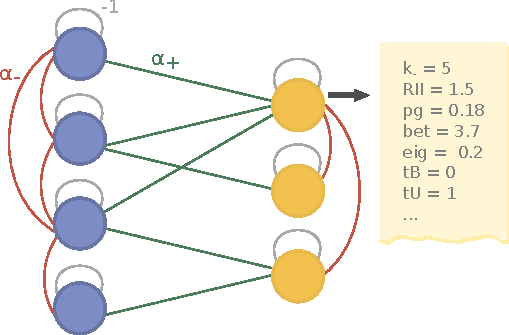
\includegraphics{figures/chp2/fig_1.pdf}
    \caption[Simple network of a community with two guilds]{Simple network of a community with two guilds (blue and yellow nodes). Species are nodes connected to themselves by gray loops, representing the regulatory effect  of  a  species  on  itself. Red links depict competitive interactions of strength $\alpha_-$ and green links refer to mutualistic interactions of strength $\alpha_+$. Competitive links have been drawn whenever two nodes in one guild share a neighbor in the opposite guild. For each node, we compute a collection of structural properties as symbolized by the yellow box. }
    \label{chp2:fig:1}
\end{figure}

\subsection{Dynamics: Replicator Equation} \label{chp2:2.2}

Once we have described the structure of the community in the previous Section,  it is the turn to define the species' dynamics. Here, our work departs from traditional approaches in which only structure is considered \cite{Allesina2009GooglingCoextinctions,Sole2001,Morone2019TheEcosystems}. Using together the structural and dynamical description of an ecological system allows  a richer discussion on how species position in the network relates to its survival. \\

The dynamics is represented by the replicator equation. This description has several advantages, the most crucial of which is that just a small number of parameters are required, contrary to other frameworks \cite{Gouveia2021,Torres-Alruiz2013AIndexes,Medeiros2021MergingSystems}. A small number of parameters allows modeling  communities with a larger number of species, a limitation of early dynamical approaches \cite{kefi2020theoretical}.  \\

The replicator equation describes the rate of change of the frequency of species $i$ in a community of $n$ species as:
\begin{equation}
    \dot{x_i} = x_i \left( \sum_j \Lambda_{i,j} x_j - \sum_{j,k} x_j \Lambda_{j,k} x_k \right).
    \label{chp2:eq:replicator}
\end{equation}
See Section~\ref{chp:methods:repli} for a complete description of the equation. In our particular case, the matrix $\Lambda$ is the adjacency matrix $A$ weighted by the interaction strength $\alpha_s$ between species. The sign of $\alpha_s$ sets the interaction type: $\alpha_+ > 0 $ for mutualism and $\alpha_- < 0 $ for competition. Combining both signs in the same system allows us to integrate different interaction types. The intraspecific entries $\Lambda_{ii}$ are fixed to $c = -1$ to facilitate the analysis, and the interspecific terms are symmetric  $\Lambda_{ij} = \Lambda_{ji}$ and equal for every pair of species  $i$ and $j$. Later on, when we add some Gaussian noise to $\alpha_s$, we will see that our result can be achieved even in the absence of symmetry (see the discussion in Figure~\ref{chp2:fig:9}). \\

The simulations start at the center of the simplex $S_n$ and finish when a stationary state is reached (see Figure~\ref{chp2:fig:3}). Specifically, we integrate the set of differential equations~\ref{chp2:eq:replicator}, where the network structure is embedded in the interaction matrix $\Lambda$. We then record the number of species that have remained alive, which is known as persistence. In practice, for computational constraints, we define a species $i$ as surviving if $x_i \geq 10^{-4}/n$. \\

\begin{figure}
    \centering
    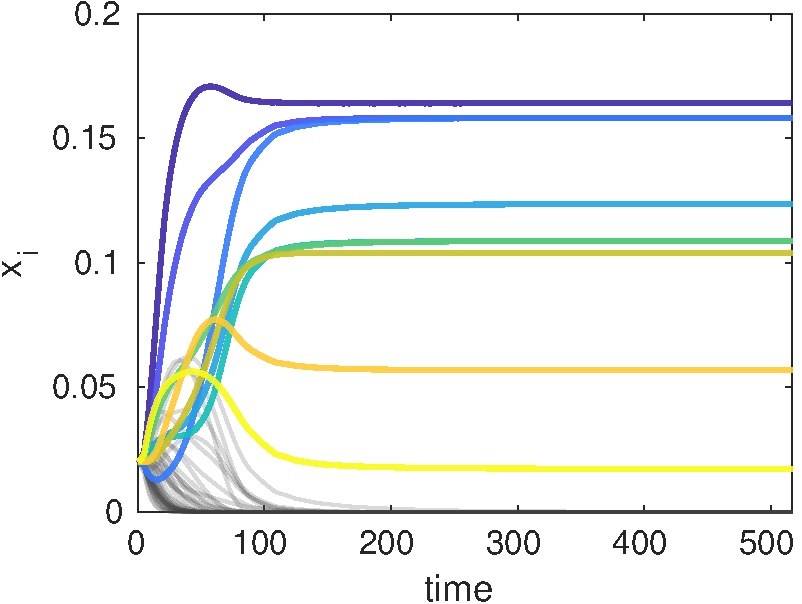
\includegraphics[width=0.7\textwidth]{figures/chp2/fig_3.pdf}
    \caption[Time evolution of mutualistic community]{Time evolution for a $50$-species mutualistic community of strength $\alpha_+ = 0.5$ in an ER graph with linking probability $p = 0.3$. At the end of the simulation, only $9$ species survive (in color), so persistence equals $18\%$.}
    \label{chp2:fig:3}
\end{figure}

The trajectories during the simulations are confined in the simplex and can settle in an equilibrium point. The equilibrium points of Eq.~(\ref{chp2:eq:replicator}) are obtained when $\dot{x}_i = 0, \, \, \forall i$. Two possible classes of solutions are found analytically: the origin (${x}^*_i = 0, \, \, \forall i$) and the values that satisfy:

\begin{equation}
    \sum_j \Lambda_{ij} x^*_j = \sum_{j,k} x^*_j \Lambda_{jk} x^*_k ,
\end{equation}
 which in turn, can be expressed as:
\begin{equation}
    \alpha_s \sum_{\substack{j \\ i\neq j} } A_{ij} x^*_j + c x^*_i = \alpha_s \sum_{\substack{j,k\\ j\neq k} } x^*_j A_{jk} x^*_k + c \sum_j x^{*2}_j
    \label{eq:solution}
\end{equation}

The equilibrium point depends on $\alpha_s$ and $c$, as well as the network structure encoded by $A$.  
If a solution has some extinct species (${x}^*_i = 0$) the right-hand side of Eq.~\eqref{eq:solution} can take any value, but it will involve $\alpha_s$, $c$, and $A$ too. Thus, as a result of describing communities as networks with embedded dynamics, the final state of a species depends on the parameters and the way in which species are connected. This setting is suitable because we want to understand how interaction patterns impact the ecological processes, eventually affecting whether or not species survive.\\

Moreover, environmental changes can alter species interactions \cite{Sun2022ExperimentalWetland,tabi2020species} and then our proxy for an environmental disruption is a global modification of the interaction strength's intensity. A community is supposed to be at its full persistence for the structures described in Subsection~\ref{chp2:2.1} for a set of interaction strength values. Then, an environmental change occurs and alters all interaction values to a new $\alpha_s$ but not the links between species. We start our simulations at that point with equal frequencies for all species and run the dynamics while tracking the species that go extinct  due to this change. Importantly, we do not remove by hand any species following the environmental change, but let the network structure affects the dynamics. We finish the simulations when a stationary state has been reached. 

\subsection{Structural Predictors: Network Metrics}  \label{chp2:2.3}

We aim to discover what are the structural characteristics that predict which species will survive. 
%In the language of complex networks, these structural characteristics are node metrics, that quantitatively capture intriguing aspects of network structure. \\

%We have chosen several candidates to test whether they are able to give us information about the survival of species.

There are many such measures, and our election has been made mainly among standard --but informative-- metrics, and structural indicators for food webs. 
%Despite it is well-known that food webs have  global structural properties that are different from those of non-trophic interaction networks \cite{Kefi2015NetworkShores,guimaraes2020structure}, the literature is biased toward food webs \cite{pascual2006ecological,kefi2020theoretical}. Since there aren't many examples of non-trophic interactions (but see \cite{Allesina2009GooglingCoextinctions, Morone2019TheEcosystems}), we also tested metrics originally associated with food webs in the hope that they might be helpful in our situation as well.\\
Since literature is biased toward food webs \cite{pascual2006ecological,kefi2020theoretical}, but see \cite{Allesina2009GooglingCoextinctions, Morone2019TheEcosystems}, we have included those predictors in our analysis despite the structural differences with non-trophic networks \cite{Kefi2015NetworkShores,guimaraes2020structure}.

Another point to consider is that species' self-regulation creates what is known in complex networks as a self-loop, a link that connects  a node to itself. Since all species have one self-loop, we have computed the metrics without taking them into account.\\

  In Table~\ref{chp:2:tab:nodeMetrics}, we present a short description where predictors are grouped together according to what structural aspect they stress. Some measures are related to the centrality of nodes, or to the analysis of groups of similar nodes within the network, and some others account for the different configurations of links.

\begin{table}[t]
\caption[Node metrics]{Node metrics. The complete list of measures with their definitions and references can be found in Appendix~ \ref{chp:methods:predictors}.}\label{chp:2:tab:nodeMetrics}
\begin{tabularx}{\textwidth}{XXX}
\hline
Centrality             & Meso-scale                              & Signed                            \\
\hline
\hline
Degree $k$             & k-core                                  & Strength                          \\
Betweenness centrality & Rich Club                               & Relative Interaction  Index (RII) \\
Closeness centrality   & Clustering Coefficient  (CC)            & Relative Balance  Index (RBI)     \\
Eigenvector centrality & Average neighbor degree  (Avg. Neig. k) & PN centrality                     \\
Pagerank               &                                         & Generalised PageRank  (GPR1)            \\
                       &                                         & Signed PageRank   (GPR2)  \\             
                       \hline
\end{tabularx}
\end{table}


\paragraph{Centrality metrics:} They describe a node's importance, i.e. its capacity to have an impact on other nodes in a network. There are several definitions of importance, so there are several descriptors \cite{Newman2010}. The simplest of all is just the number of links connected to a node, i.e. the degree $k$. If we want to take the importance of the node's connections into account, the eigenvector centrality gives a centrality score proportional to the centrality of the neighbors. In a variant called PageRank, the centrality of a node is primarily proportional to the centrality of the neighbors but divided by their degree.

 Alternative formulations of centrality are based on paths. For example, betweenness centrality measures to what extent a node is located on pathways between other nodes, and closeness centrality assumes that a central node has a low average distance from other nodes.

\paragraph{Meso-scale metrics:} Quasi-local properties provide an intermediate description level by grouping nodes. As with the concept of importance, here we also face different working definitions for \textit{groups}. The k-core is one of these  metrics \cite{Morone2019TheEcosystems}. It is a set of nodes where each is connected to at least $k$ others. 

When there are no genuine groups but rather certain ways in which nodes are connected, we can measure the clustering coefficient $CC$ or the average neighbor degree. The $CC$ quantifies the level of transitivity of a node as the fraction of the neighbors that are themselves neighbors.

\paragraph{Signed metrics:}Finally, some of these properties can be generalized to include information about the sign of the interactions involved. Since our main objective is to model communities with mutualistic and competitive interactions, a natural property of the nodes is the degree of each type of interaction. For example, the competitive degree $k_-$ is the number of species with which a species is competing. To also consider the magnitude of the interactions, we define the strength of a node as the sum of the interaction strengths of its links. Other more complex metrics have been borrowed from social sciences such as the PN centrality and two generalizations of the PageRank have been developed for this study.

\subsection{Metrics' importance: Decision Trees} \label{chp2:2.4}
A common but arduous challenge in network science is to relate the dynamics on a network with its structure \cite{Newman2010,Holme2021NetworksConsequences}. Here, we face that challenge because we seek properties (structure) that determine the fate of a species (dynamics). Among the aspects that involve both the dynamics and the network structure, some are more well-suited to be treated analytically --like stability-- and others that don't. Our research question falls in the latter case due to the complexity of ecological networks, and hence we need another approach to classify  surviving species according to their structural features and find the most relevant of those features. Fortunately, machine learning classifiers can do precisely that.  \\

We have used a machine learning algorithm called Decision Trees,  whose fundamentals are explained in Appendix~\ref{appen:DT}. Decision trees generate a set of rules to predict the correct class of an observation from a set of variables. The rules are nominal yes/no questions about the properties of the variables.  \\

In our particular case, the observations are species and the classes are their state at the equilibrium, which is ``Surviving'' or ``Extinct''. For each community, we train a decision tree with that information and the initial node metrics as the set variables (see yellow box in Figure~\ref{chp2:fig:1}a).  The decision tree discriminates which species survive according to the values of some of the metrics. A tree whose root node is the competitive degree $k_-$ is depicted in Figure~\ref{chp2:fig:2}. This toy tree classifies species only based on four different metrics: $k_-$, Relative Interaction Index ($RII$), PageRank, and betweenness centrality.  Each node of the tree checks the value of one metric. Having a particular species in mind, the first decision to be made is whether its $k_-$ exceeds $3$. If not, we follow the left branch, and we see that the tree classifies the species as ``surviving''. If, however, it is smaller than $3$, we follow the right branch to the next node. Here, the tree asks if the $RII$ of the species is smaller than $0.5$. In this way, we will navigate the tree until we land on the corresponding leave. \\

\begin{figure}[t]
    \centering
    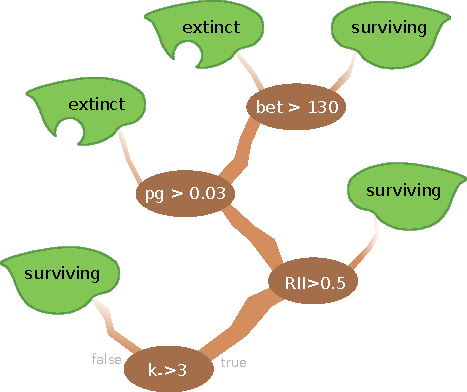
\includegraphics{figures/chp2/fig_2.pdf}
    \caption[Schematic diagram of a decision tree]{Schematic diagram of a decision tree. It has four nodes: competitive degree ($k_-$) as the root node, Relative Interaction Index ($RII$), PageRank ($pg$) and betweenness centrality ($bet$). These node metrics are the ones chosen during the training as the most useful to classify the species of an imaginary community. The threshold values are only for illustrative purposes.}
    \label{chp2:fig:2}
\end{figure}

To test the accuracy of the decision tree, we can cast a glance at the confusion matrix, which presents the percentage of correct and incorrect classifications (Figure~\ref{chp2:fig:6}a  as well as in Figure~\ref{chp2:fig:8}). For example, in Figure~\ref{chp2:fig:6}a, the decision tree for $\texttt{Emp}$\_$\texttt{IL}$ classifies with $99.5\%$ sensitivity that an extinct species actually goes extinct and with $99.2\%$ specificity that a surviving species will survive. False positives (extinct species predicted to survive) and false negatives (surviving species labeled as extinct) are very low, $0.5\%$ and $0.8\%$ respectively. \\

An accurate decision tree will find among all the proposed structural node properties the most relevant ones, which will be called \textit{structural predictors}. The importance profile (see e.g. Figures~\ref{chp2:fig:5}  and \ref{chp2:fig:7}) displays the quantitative importance of each potential predictor based on the definition of importance given by Eq.~\eqref{eq:importance}. The structural predictors stand out as the properties with systematically higher importance among the different structures. \\

Finally, to further test the generality of the predictors for each interaction type, we will modify some characteristics of the communities and train a decision tree for each new scenario. In particular, we will vary the interaction strength $\alpha$ (Figure~\ref{chp2:fig:4}), add noise to its value (Figure~\ref{chp2:fig:9}) and perform simulations with diverse network structures
%%%%%%%%%%%%%%%%%%%%%%%%%%%%%%%%%%%%%%%%%%%%%%%%%%%%%%%%%%%%%%%%%%%%%
\section{On the brick: results of structural predictors step by step}


%\paragraph{(moti+what)} First, we simulate communities with only one type of interaction as the first step towards combining  both competition and mutualism. Given that environmental changes alter species interactions \cite{Sun2022ExperimentalWetland}, and this in turn can cause extinctions, we start studying  how exactly the persistence varies with the strength of the interactions $\alpha$. 

Once the methodology and scope have been defined, we start to build intuition about the results we are going to find. We begin simulating communities with only one type of interaction as the first step towards combining both competition and mutualism. By doing so, we mirror the traditional approaches in which networks only describe one ecological process, and check if our results are consistent with the previous literature. The results obtained in this situation will help us to better understand the implications of taking several interactions simultaneously. 

\subsection{Persistence and interaction strength}
Given that environmental changes alter species interactions \cite{Sun2022ExperimentalWetland,tabi2020species}, and this, in turn, can cause extinctions, we start studying  how exactly the persistence varies with the strength of the interactions. More precisely, we increase the interaction strength as a proxy of the environmental change and record the species that perish. Since our dynamical model has few parameters by construction, we go ahead studying how persistence varies with the strength of interactions $\alpha_+$ on one side and  $\alpha_-$ on the other. We simulate communities for all the network structures of Section~\ref{chp2:2.1}, varying $\alpha_s$ by several orders of magnitude, and measuring the final percentage of surviving species. 
As a technical note, the artificial networks have been constructed in such a way that they have the same connectance as the empirical ones.  For the latter, we only take the links that correspond to the interaction type being studied. For example, if we focus on mutualism, the community of Figure~\ref{chp2:fig:1} will have solely green and gray links.\\

\begin{figure}[t!]
    \centering
    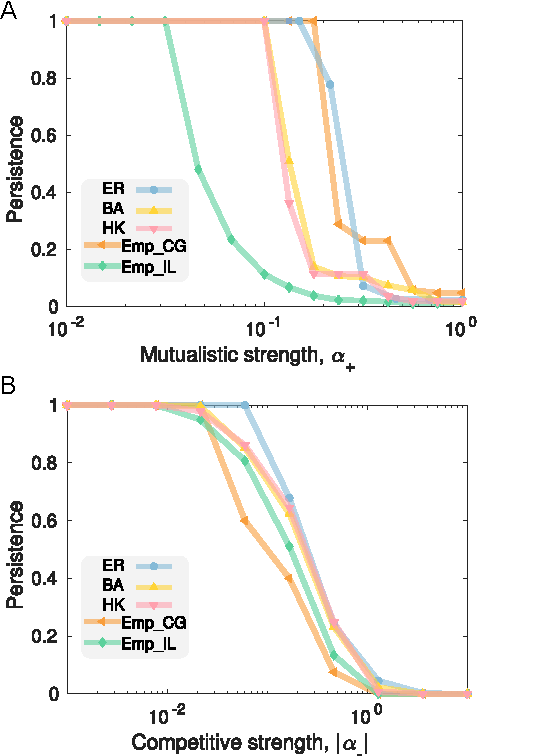
\includegraphics[width=0.6\textwidth]{figures/chp2/fig_4.pdf}
    \caption[Impact of interaction strength on persistence]{ Persistence decreases with high  interaction strength in absolute value for all network models. For illustrative purposes, only the largest empirical network of each type is displayed. Type (A) is represented by the pollinator network
 $\texttt{Emp}$\_$\texttt{IL}$ \cite{robertson1928flowers}. It has a total  of $n = 1500$ species, $456$ plants, and their $1044$ pollinators. Type (B) is $\texttt{Emp}$\_$\texttt{CG}$, a $104$ plant-species network extracted from \cite{Saiz2017EvidenceNetworks}. The random models have been simulated $10$ times for each value of $\alpha_s$, created  with $n = 500$ and a connectance $C$ equal to $\texttt{Emp}$\_$\texttt{IL}$ ($C_{mut} = 0.014$, $C_{com} = 0.012$). (Panel a) Mutualism. ER: $p =  0.009$; BA: $m_{links} = 2$; HK: $m_{links} = 2$, $p_t = 0.4$,  (Panel b) Competition. ER: $p =  0.1$; BA: $m_{links} = 30$; HK: $m_{links} = 30$, $p_t = 0.7$.}
    \label{chp2:fig:4}
\end{figure}

A smaller number of species survives as the absolute value of the interaction strength increases for both interactions and all network constructions, as shown in Figure~\ref{chp2:fig:4}. Networks simply differ in terms of when the transition happens, although  the critical value is rather similar. For instance, in Figure~\ref{chp2:fig:4}b, the lines for the BA and HK models are superimposed. This result falls into the traditional understanding of community ecology, where strong interactions lead to smaller or unstable communities \cite{May1972WillStable}, or smaller feasibility domains \cite{Grilli2017}. \\

After this result, we can assure that our proposed structures and dynamics work as expected and now proceed further to check the possible predictors. To do that, we choose an interaction strength that gives us a persistence of around $50\%$ to prevent biases in the training of the decision trees (see Section~\ref{chp2:2.4} and Appendix~\ref{appen:DT} for more insights about decision trees and  Appendix~\ref{SI:1} for cases where persistence is not equal to  $50\%$). \\

To understand the effects of multiple interactions within the same community, we start by studying mutualistic and competitive networks separately. In both cases, we set a network structure and measure the initial node properties for each species. After simulations reach the equilibrium, a decision tree is trained. It is fed with the node properties and a boolean variable that encodes whether the species is alive at the end of the simulation or not. Finally, we obtain the relative importance of those metrics in predicting survival, which is explained in Appendix~\ref{appen:DT}. \\

\subsection{Mutualistic networks}

For all network types with mutualistic interactions, the most important node property is eigenvector centrality, as can be seen in Figure~\ref{chp2:fig:5}a for artificial networks and in Figure~\ref{chp2:fig:5}b for empirical networks. Furthermore, the accuracy of the prediction is high as shown in the confusion matrix of Figure~\ref{chp2:fig:6}a. We can therefore conclude that the decision tree is well-trained, and we observe that it points to eigenvector centrality as the main predictor of extinction after an environmental change for mutualistic networks. \\

\begin{figure}
    \centering
    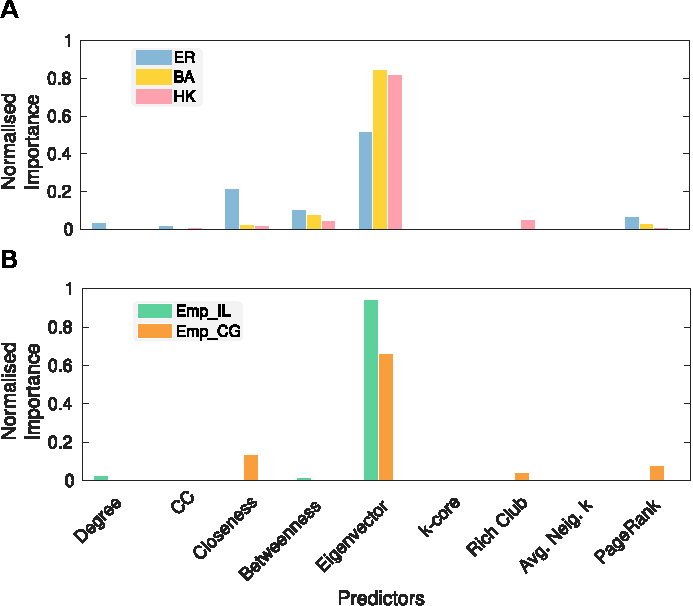
\includegraphics{figures/chp2/fig_7.pdf}
    \caption[Importance profile for mutualism]{When communities are purely mutualistic, the most important predictor for all network structures and interaction strengths is eigenvector centrality. The importance profile is in Panel a, where the normalized importance of each predictor  is plotted for artificial 500-node networks. ER: $p =  0.009$, $\alpha_+ = 0.22$; BA: $m_{links} = 2$, $\alpha_+ = 0.14$; HK: $m_{links} = 2$, $p_t = 0.4$, $\alpha_+ = 0.12$. (Panel b) Normalized importance for empirical networks from the three different datasets' collections. (type A) $\texttt{Emp}$\_$\texttt{IL}$: $N = 1500$, $\alpha_+ = 0.4$; (type B) $\texttt{Emp}$\_$\texttt{CG}$: $N = 104$, $\alpha_+ = 0.2$.}
    \label{chp2:fig:5}
\end{figure} 

Next, we plot the eigenvector centrality of the species at the beginning of the simulation versus their extinction time. We do this because the decision trees have determined that this type of centrality is the best one to classify whether a species becomes extinct. Eigenvector centrality is hence expected to correlate in a meaningful way with the fate of the species. From Figure~\ref{chp2:fig:6}b, we observe that the species that are worse connected, in terms of their eigenvector centrality, become extinct earlier. This tendency helps us to find the coherence behind the predictor, with the following narrative:

\begin{figure}[t]
    \centering
    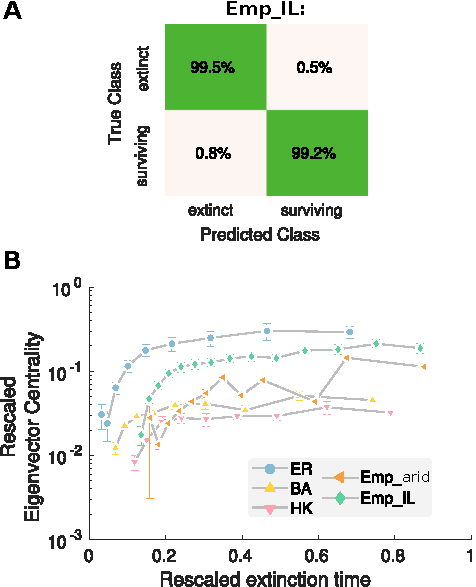
\includegraphics{figures/chp2/fig_6.pdf}
    \caption[Confusion matrix and time evolution of the eigenvector centrality in mutualistic communities]{(Panel a) The confusion matrix of one empirical network exemplifies the goodness of the trained Decision Trees. (Panel b) The initial eigenvector centrality plotted versus the time at which species become extinct reveals a pattern: species with low eig. centrality tend to die earlier. For clarity, the value for each point is the average eig. centrality of extinct species at nearby times. The same graph without binning is in Figure~\ref{chp2:fig:SI2_mut} of Appendix~\ref{appen:SuppPredictors}.}
    \label{chp2:fig:6}
\end{figure}

According to equation Eq.~(\ref{chp2:eq:replicator}), having more neighbors with positive $\alpha$ increases the local fitness and, consequently, we expect a centrality measure to take the main role in predicting survival. If a species has low eigenvector centrality, it is poorly connected and consequently has lower fitness. Moreover, eigenvector centrality grants a score proportional to the scores of the neighboring species, so a low value is an indicator that the mutualistic partners of the species are themselves performing badly. These species could not overcome the average fitness of the total community and hence become extinct. \\

Even for different types of networks, our result is in line with the literature and with what we expected. For instance, the fact that eigenvector centrality can rank the importance of species has already been found, but in the context of the collapse of food webs \cite{Allesina2009GooglingCoextinctions}. In mutualistic networks, there is still another reason that favors the role of centrality. One well-known property of these networks is their heterogeneity in the number of links: there are generalists and specialists species\cite{bascompte2003nested}. As a consequence, centrality metrics greatly vary among species and stand out as a distinctive characteristic. Moreover, although this structural regularity is reported for real-world networks, it is remarkable that the main predictor and the form of the curves in Figure~\ref{chp2:fig:6}b  are common to all types of structures, artificial as well as empirical. \\
 

\subsection{Competitive networks}
In this case, all the interaction strengths among species are negative. Taking a look at the mathematical form of local fitness in Eq.~\eqref{eq:localfitness}, a species with lots of competitors --more neighbors-- will have a lower fitness since the addends are negative. Thus, this causes its density to decrease faster. Accordingly, we expect again a centrality measure to play an important role in survival. \\

The trained decision tree reveals that the most important predictor, in this case, is  PageRank (Figure~\ref{chp2:fig:7}), again for both artificial (Panel a) and empirical networks (Panel b). The prediction has high accuracy too (Figure~\ref{chp2:fig:8}a).\\

Contrary to positive interactions, having high centrality is detrimental in competitive networks. And as a consequence, in Figure~\ref{chp2:fig:8}b, we observe that the species with  larger PageRank are the ones that became extinct first. Nevertheless, PageRank and eigenvector centrality are two very similar metrics, in the sense that both assign a score following the neighbors' centrality ratings \cite{Newman2010}. \\
 
\begin{figure}
    \centering
    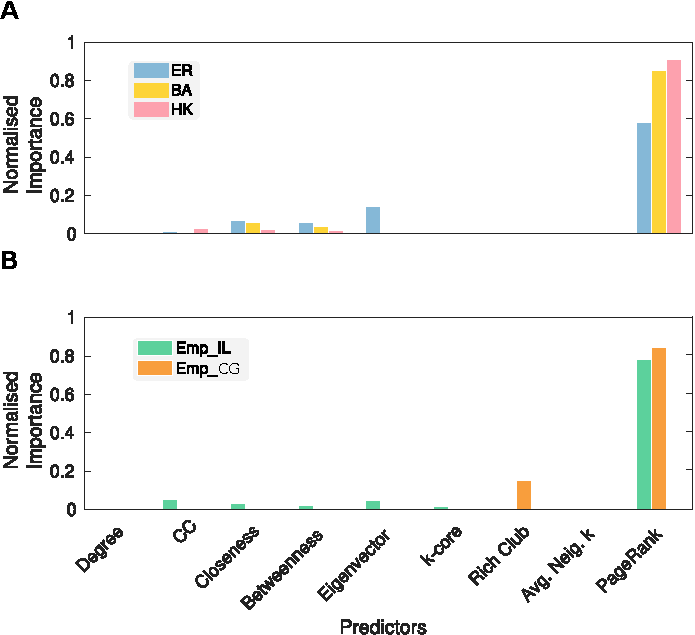
\includegraphics{figures/chp2/fig_5.pdf}
    \caption[Importance profile for competition]{In a community with only competition, the most important predictor for all network structures and interaction strengths is PageRank. The importance profile is in (Panel a), where the normalized importance of each predictor  is plotted for artificial 500-node networks. ER: $p =  0.009$, $\alpha_- = 0.45$; BA: $m_{links} = 2$, $\alpha_- = 0.4$; HK: $m_{links} = 2$, $p_t = 0.4$, $\alpha_- = 0.35$.  (Panel b) Normalized importance now for empirical networks from the three different datasets' collections: (type A) $\texttt{Emp}$\_$\texttt{IL}$: $N = 1500$, $\alpha_- = 0.25$; (type B) $\texttt{Emp}$\_$\texttt{arid}$: is the combination of all competitive networks in this collection because they were individually too small.}
    \label{chp2:fig:7}
\end{figure}

\begin{figure}
    \centering
    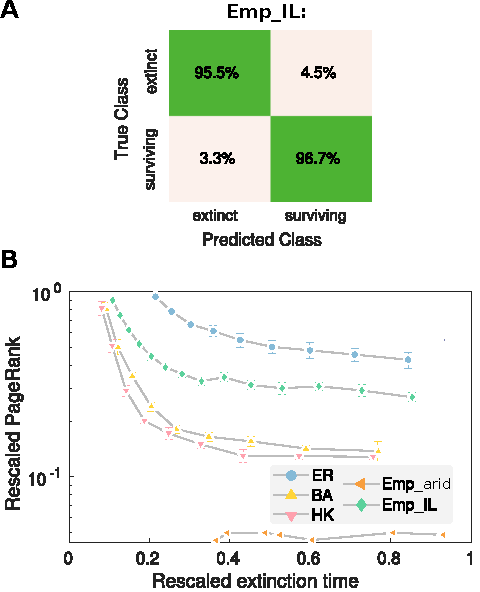
\includegraphics{figures/chp2/fig_8.pdf}
    \caption[Confusion matrix and time evolution of PageRank in competitive communities]{(Panel a) The confusion matrix of one empirical network exemplifies the goodness of the trained Decision Trees. (Panel b) The initial PageRank of each species plotted when it becomes extinct reveals a pattern: the species with high PageRank tend to die earlier. For clarity, the value for each point is the average Pagerank of species extinct at nearby times. The same graph without binning is in Figure~\ref{chp2:fig:SI2_comp} of Appendix~\ref{appen:SuppPredictors}. }
    \label{chp2:fig:8}
\end{figure}

Additionally, while the number of coexisting species varies with the intensity strength --the intensity of the environmental change--, the main predictors do not when only one interaction type is considered. The main predictors also remain the same when $\alpha_s$ is set as a baseline value plus some Gaussian noise, $\alpha'_s  = \alpha_s + \mathcal{N}(0,\sigma^2)$. In Figure~\ref{chp2:fig:9}, we can see that even when the noise has a standard deviation of the same magnitude as the strength itself, eigenvector centrality and  PageRank obtain the highest importance again. All these facts highlight the robustness of eigenvector centrality and PageRank as the main predictors for mutualistic and competitive networks, respectively. \\

\begin{figure}[t]
    \centering
    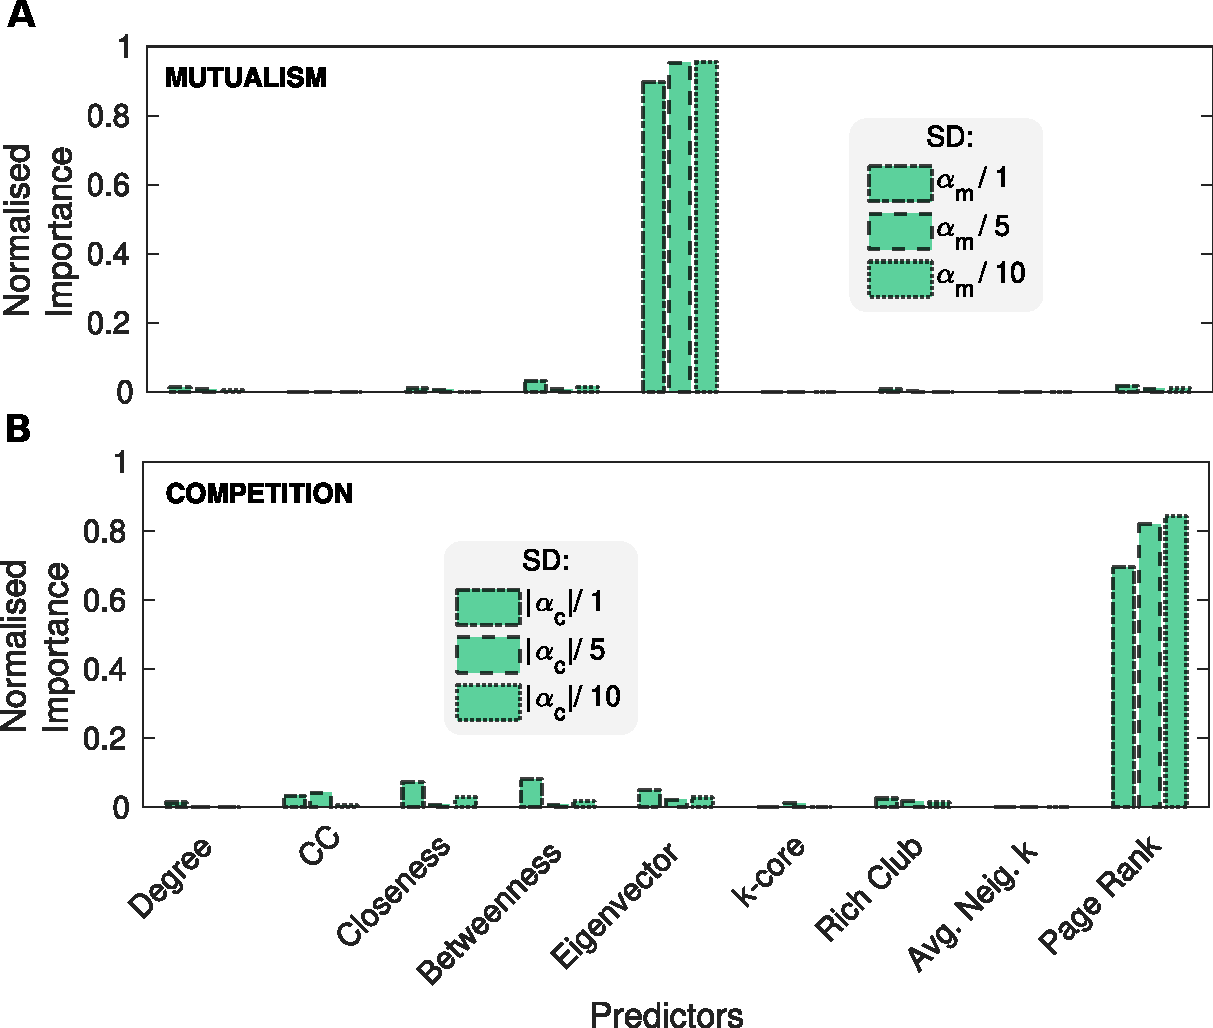
\includegraphics[width=\textwidth]{figures/chp2/fig_9.pdf}
    \caption[Importance profile with Gaussian noise]{The importance is not modified when we add Gaussian noise to the values of $\alpha$. SD stands for standard deviation. (Panel a) $\alpha_m = 0.04$ (Panel b) $\alpha_c = -0.2$. The network is $\texttt{Emp}$\_$\texttt{IL}$. }
    \label{chp2:fig:9}
\end{figure} 

 To summarize our results so far, we have studied one interaction type at a time after an environmental perturbation and, as a novelty, related the node properties of the species in the network with its final state after a simulation in simple dynamics, using a machine learning classifier. We have obtained that a single structural metric contains all the necessary information to predict whether a species will survive or not given its place on the network. This metric is eigenvector centrality for mutualistic networks, and PageRank for competitive networks. Importantly, these metrics continue to be the main predictors for different values and levels of noise of the interaction strength (i.e. of  persistence), and in all network structures that we have simulated. This suggests that the fate of the species depends heavily on their neighborhood and less on the overall network structure.
 
\subsection{Predictors in the presence of both types of interactions}\label{chp:2:3:4}

Once we have determined the predictors for only mutualistic or only competitive networks, we are ready to study communities with multiple interactions. We wonder whether the results for single-interaction communities hold, namely that solely one predictor is necessary to correctly classify the species, which in turn would be centrality-based and robust to changes in the intensity of interactions and network topology. In this case, we simulate communities with mutualistic and competitive interactions at the same time. \\

Adding a second type of interaction increases the complexity of the system, and so does the number of parameters to be chosen (number of mutualistic/competitive links, relative interaction strengths, etc).  We have thus introduced $\rho$, the ratio between competitive $\alpha_-$ and mutualistic $\alpha_+$ strength, to relate the interactions' strengths. Initially, it is set to $one$ to compare all the networks. For the same reason, we have only simulated real-world networks and not artificial ones. In that way, the percentage of positive and negative links in the networks and their distribution among species are based on empirical findings.\\

Comparing the effect of the real-world structure with a null model is now done via reshuffling (Section~\ref{chp:methods:networks}). We create alternative networks where overall characteristics such as the connectance and degree distribution of the empirical network are conserved, but the exact interacting patterns change at random. In that way, we could distinguish whether the future predictors depend on general average properties of the networks or on the particular way species connect. \\

The set of potential predictors is updated with signed metrics --as networks have now signed links. These metrics include information not only on structural properties but on the signs and strengths of the interactions (recall  Sections~\ref{chp2:2.3} and Appendix~\ref{chp:methods:predictors}). \\

Figure~\ref{chp2:fig:11} reveals the predictors obtained through the decision trees for our two types of empirical networks. There are several points at which the results of Figure~\ref{chp2:fig:11} differ from single-interaction networks. First notice that there is not a clear unique predictor. The highest importance is not as high as in the cases of only one type of interaction. Now we have other node properties that also have non-negligible importance. Regarding these properties,  they are mainly the metrics that take the sign of the interaction into account, especially PN centrality and PageRank's generalizations. Finally, and maybe this is the most intriguing of all the differences, the set of predictors varies from network to network. With two interactions, we lose the regularities found with just one interaction. Several metrics are needed to correctly classify species, whose identity and importance vary with the datasets. \\

\begin{figure}[t]
    \centering
    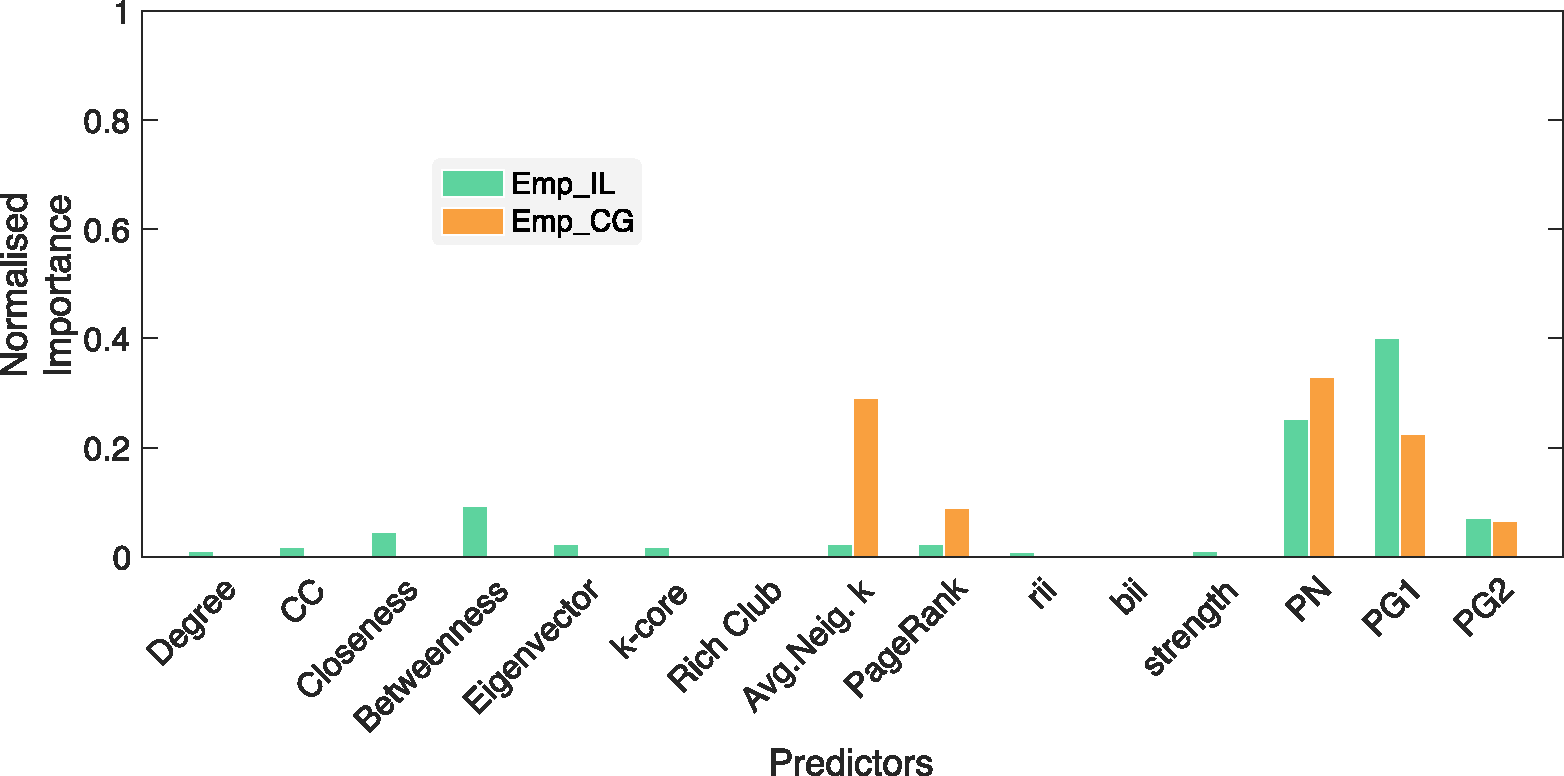
\includegraphics[width=1.05\textwidth]{figures/chp2/fig_11.pdf}
    \caption[Importance profile with several types of interactions at the same time]{The importance profile when mutualism and competition are studied simultaneously varies from network to network. For $\texttt{Emp}$\_$\texttt{IL}$ the parameters of the simulation are $\alpha_+ = \alpha_- = 0.14$ ($\rho = 1$). For $\texttt{Emp}$\_$\texttt{CG}$, $\alpha_+ = \alpha_-  = 0.18$ ($\rho = 1$).}
    \label{chp2:fig:11}
\end{figure}

To further examine the causes behind this divergence, we first explore the space of values of $\rho$ to test whether different strength ratios --and hence different environmental disruptions-- limit the range of predictors that are observed across different communities. Previously, the ratio had been set to one in Figure~\ref{chp2:fig:11} for simplicity, meaning that competition and mutualism have the same strength. We are interested in whether communities with a dominant interaction share similar predictors, which could suggest relative strength is a strong determinant of the predictors. Figure~\ref{chp2:fig:12} presents the importance profiles for several simulations of the same empirical network with different values of $\rho$, in particular when competition is five times stronger and weaker than mutualism. We observe that the set of predictors changes. Their importance is altered and even new predictors appear for some particular $\rho$ --a clear example is the closeness centrality for $\rho = 1/5$. Therefore, the predictors depend on the relative values of the interactions and, ultimately, this means that the internal dynamics embedded in the network affect them. \\

Then, we compare the importance profiles of our empirical networks with equivalent reshuffled networks maintaining the same interaction strengths. By confronting these random networks with the empirical ones, we can determine the role that interactions not placed at random have. Figure.~\ref{chp2:fig:13} shows that the predictors' importance changes and, given the error bars, the divergence can be large. Moreover, since the importance profile is not fully conserved after a notably conservative reshuffling, we can deduce that the predictors also depend to some extent on network structure. \\

\begin{figure}[t]
    \centering
    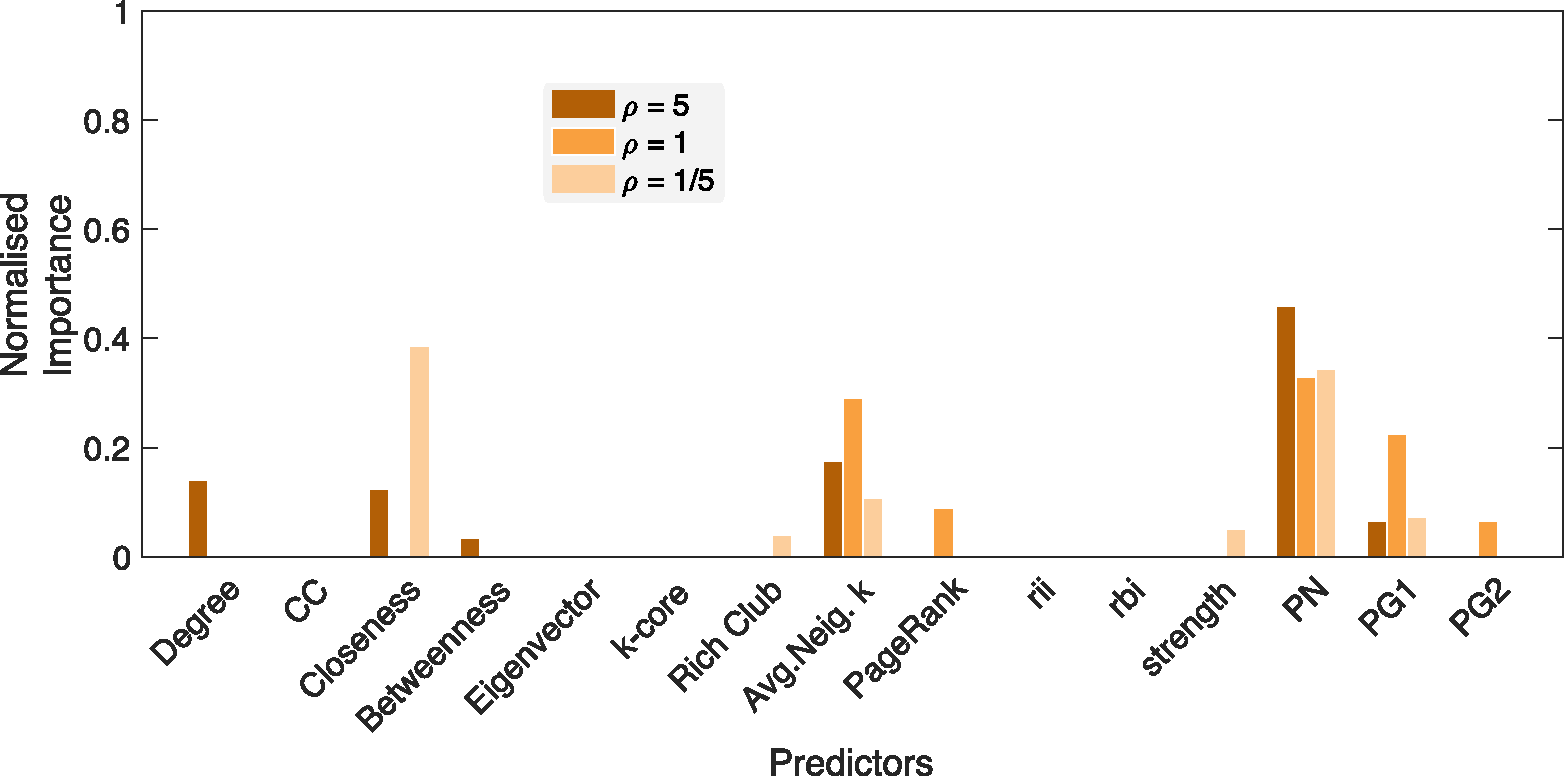
\includegraphics[width=1.05\textwidth]{figures/chp2/fig_12.pdf}
    \caption[Impact of the interaction strengths' ratio on the importance profile]{Changes on the importance profiles of the same network with different parameters. The system is $\texttt{Emp}$\_$\texttt{CG}$, where the setting for $\rho= 1$ is the same as in Figure~\ref{chp2:fig:11}. }
    \label{chp2:fig:12}
\end{figure}

 \begin{figure}[t]
    \centering
    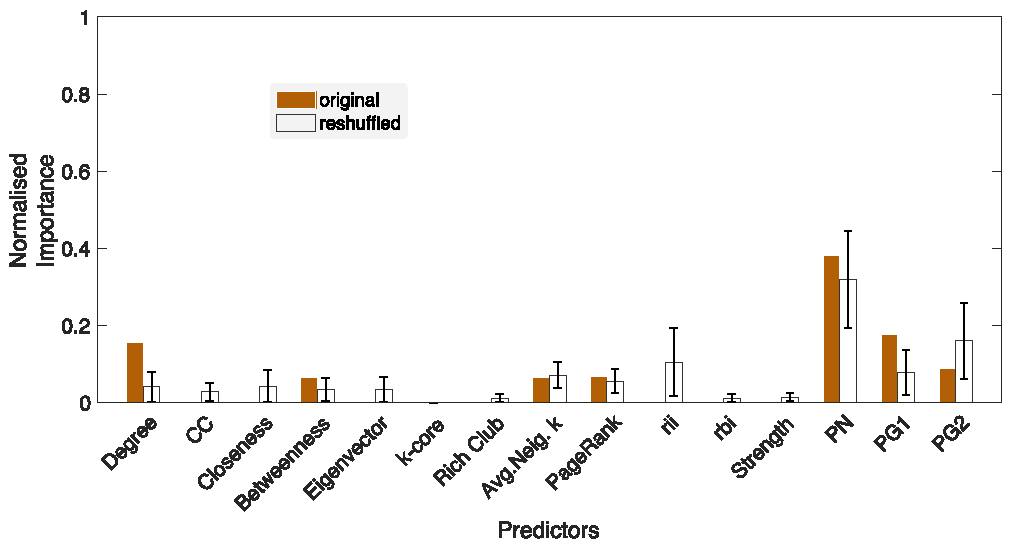
\includegraphics[width=1.05\textwidth]{figures/chp2/fig_13.pdf}
    \caption[Impact of reshuffling on the importance profile]{ Comparison between the importance profile of a network and their reshuffled versions. The importance of each predictor is averaged over $10$ reshuffled networks with the same dynamical parameters, and error bars mark the mean standard deviation. The original system is $\texttt{Emp}$\_$\texttt{CG}$ with $\rho = 5$ from Figure~\ref{chp2:fig:12}. }
    \label{chp2:fig:13}
\end{figure}

\begin{figure}
    \centering
    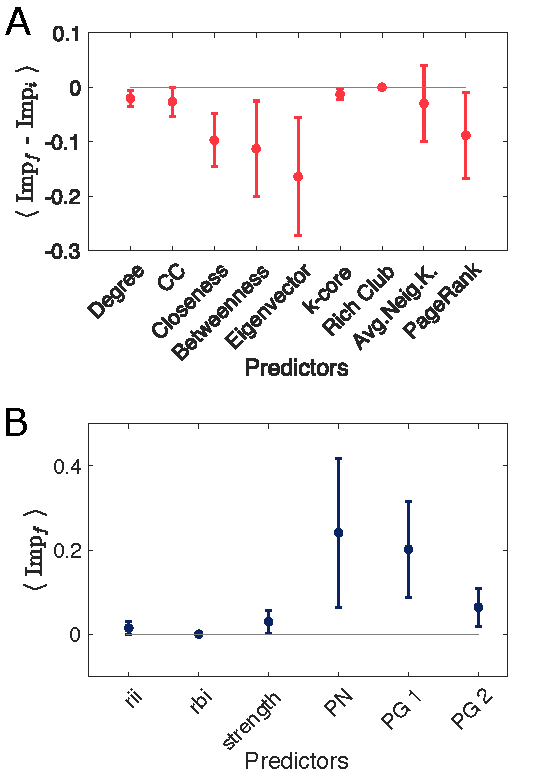
\includegraphics[width=.7\textwidth]{figures/chp2/fig_1415.pdf}
    \caption[ \, Differences on the importance for unsigned and signed predictors]{(Panel a) Average difference in importance for unsigned predictors before ($\texttt{Imp}_i$) and after  ($\texttt{Imp}_f$) adding signed metrics to the decision trees' training sets. The networks are the nine empirical networks described in \ref{tab:empnetworks}. (Panel b) Average importance of signed metrics over the same empirical networks. For all metrics, except average neighbors degree (Avg.Neigh.k.) in Panel a, the confidence intervals do not cross the horizontal axis. We can then conclude that the decrease in the importance of unsigned metrics as well as the non-zero importance of some signed metrics are significant.}
    \label{chp2:fig:1415}
\end{figure}

 We have just concluded that, when a system is described by more than one type of interaction, it cannot be characterized by a single predictor. The decision tree is not able to consistently find a main predictor for both interactions, even though it gets good results with the interactions in isolation. Worst still, one might think that \textit{the} important property is actually missing from the pool of potential predictors. Nevertheless, the sensitivity to the strength of interactions, and the fact that a given set of predictors varies with a subtle reshuffling suggest that there isn't any. \\

Eigenvector centrality and PageRank do not frequently appear as important when we study communities with both types of interactions. Instead, other metrics that record centrality influenced by the sign of the interactions become more relevant. The stability of communities cannot be predicted by simply adding what we already know from studying separately mutualism and competition. The combination of mutualistic and competitive interactions results in complex behavior. \\

The previous findings highlight the urgency of studying each community independently, as there is no robust, unique predictor. A particular distribution of interactions and their strengths seem to fix the important metrics, which change from case to case.   Nevertheless, we can still get some general results for multiple-interaction networks. \\

We can anticipate the most probable predictors because the signed metrics have appeared more frequently than other potential predictors, as it is seen in Figures~\ref{chp2:fig:11}, \ref{chp2:fig:12} and \ref{chp2:fig:13}. To strengthen this statement, we systematically average the importance of each predictor over all our empirical networks. We start by comparing the mean importance obtained by unsigned metrics before and after introducing signed metrics in the training set. The importance of the former decreases significantly (Figure~\ref{chp2:fig:1415}a) when signed metrics are also present in the training. Further, the mean importance of signed metrics is plotted in Figure~\ref{chp2:fig:1415}b. Several values are non-negative, indicating that they are important on average. Among them, PN centrality has the highest importance, followed by the generalizations of PageRank. These plots can be interpreted as follows: predictors based on the structure and dynamics of a system get higher importance because they contain more information about the fate of its species. A more complete knowledge of species dynamics is needed to evaluate species risks. Knowing only the structure is not enough.\\

The centrality of a species still plays a role, since  PN centrality and generalizations of PageRank are still based on how pivotal a species is. But being in some way central is not a sufficient indicator anymore. The number of mutualistic and competitive neighbors, and how strong these interactions are, also play a role. These two facts vary enormously among networks (see Table~\ref{tab:empnetworks}), preventing the decision tree from finding universal predictors.\\

\section{Discussion and perspectives} \label{chp2:4}

Protecting vulnerable species from extinction is crucial for conserving the planet. Apart from blatant cases, how to sort species in a community according to their extinction risk is an open problem. One fruitful approach is to make use of a network representation of the ecological relationships species participate in \cite{pascual2006ecological}. Traditionally, these networks describe only one type of interaction in isolation, and artificially remove species without modeling their abundances \cite{Sole2001}. Here, considering simple dynamics with both mutualism and competition, we have found that the regularity and predictability that hold for mutualism and competition when studied separately no longer apply. \\

We have started our work finding a node metric that predicts what species are going to become extinct first after an environmental change when only one type of interaction is present. Using a machine learning classifier, we have found that the species that survive in only mutualistic networks are the ones with the highest eigenvector centrality. We have obtained an equivalent result for only competitive communities, where species perish first if they have high values of PageRank. However, in ecological networks simultaneously including both interactions, species are no longer characterized by a local structural property. Including dynamical factors like the strength of their interactions enhances survival prediction. \\
%Furthermore, communities with more than one interaction are  described by a unique set of metrics. \\

A direct consequence of these results is that a species that was predicted to be thriving according to its mutualistic interactions may not be that safe. The predictors that determine safety vary when we add information on competitive interactions. In addition, we cannot ultimately anticipate the new set of predictors since they vary from network to network and with interaction strength.  And ultimately, we may not have complete information on the present interactions and their strengths --certainly not all of them. \\

This lack of universality contrasts with the regular patterns found when only one type of interaction is considered in our model and the literature. For example,  k-core is thought to be a predictor of structural collapse in mutualistic ecosystems \cite{Morone2019TheEcosystems}. Would this prediction change if competition was  added to the study? Seminal works have taught us that the architecture of ecological networks may be the result of the interweaving effect of several interactions. This is the case of the ubiquity of the nestedness, a main highlight of the architecture of mutualistic networks, that  minimizes competition and increases
biodiversity \cite{bastolla2009mutualism}.\\ 

 We have only studied mutualism and competition in the present work. The reason behind this choice is the proposed balance effect that the two interactions have on ecosystems \cite{bastolla2009mutualism,Wang2021InterspecificNetworks, Gracia-Lazaro2018TheEcosystems}. A natural question that arises is whether our results can be extended to communities with other interactions. Our methodology is ready to be applied to combinations of other kinds of non-trophic interactions such as parasitism \cite{dominguez2021structure, pilosof2017multilayer}, or in food webs \cite{Garcia-Callejas2018ThePersistence,Garcia-Callejas2021TheConstraints}.  \\

Finally, we have only presented here results that are oriented towards the prediction of survival after a change in parameters since that was our main objective. Still, the model has an interesting behavior by itself and calls for more systematic studies to unveil the interplay between structure and dynamics. For example, the impact of the ratio of interaction strengths on persistence, or how predictors change when the dynamics are refined to Lotka-Volterra equations with allometric coefficients. \\

% TO CONCLU: As a take-home message, when we study communities with both types of interactions, predictors are not universal and vary with the structure of each community and the interaction strengths. As a consequence of the results of this work, we are now in a position to highlight the significance of revisiting classic results of interactions in isolation, which bring us closer to the ultimate challenge of studying several interactions simultaneously to better understand ecosystems.

%Many efforts are made to allocate resources for conserving the planet. One approach is to protect certain species that are considered key players for the heath of an ecosystem. How to identify these species is, however, still far to be settled. An intuitive way to assign importance 
%Each community is unique. In addition, the importance of node characteristics depends not only on network structure, but on the strength and sign of the interactions. 
